% Created by tikzDevice version 0.7.0 on 2014-08-02 12:32:26
% !TEX encoding = UTF-8 Unicode
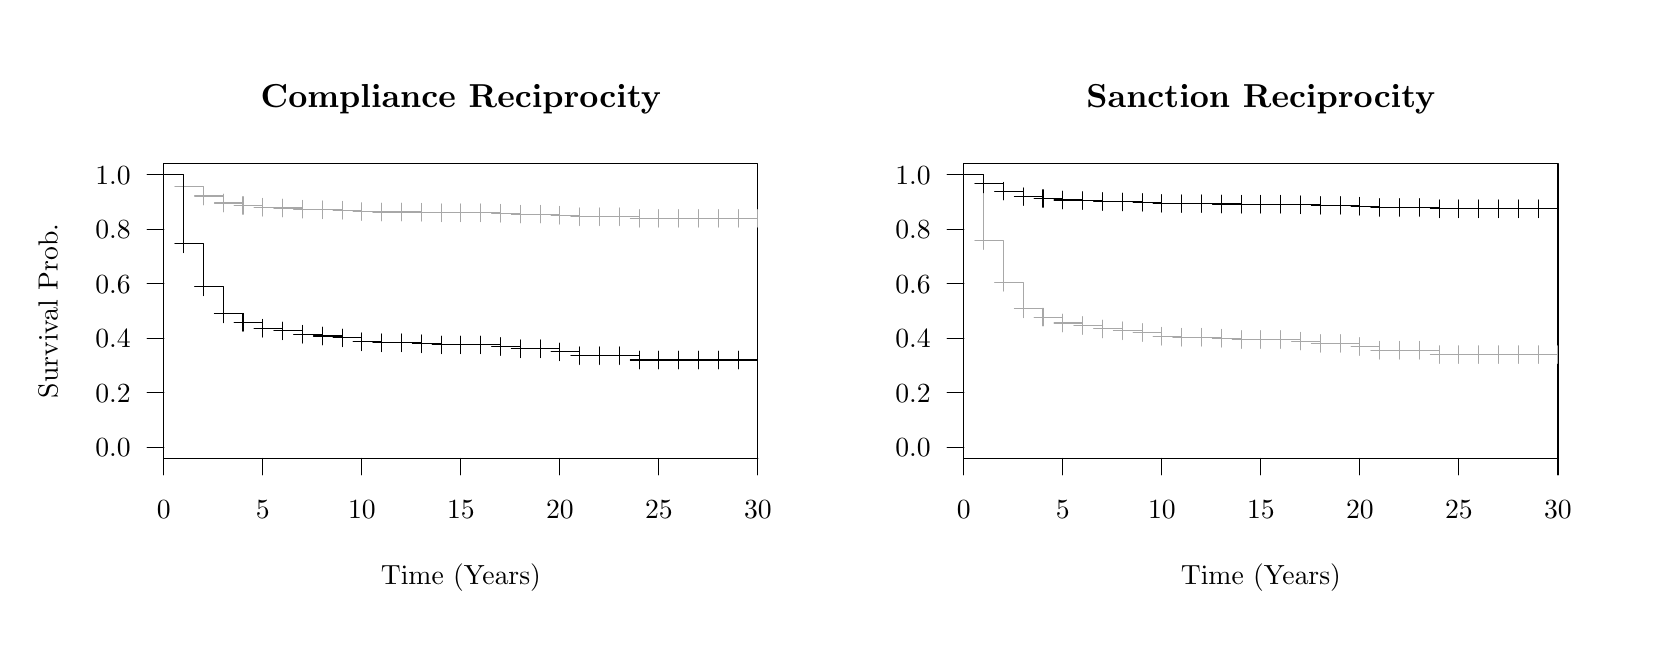
\begin{tikzpicture}[x=1pt,y=1pt]
\definecolor[named]{fillColor}{rgb}{1.00,1.00,1.00}
\path[use as bounding box,fill=fillColor,fill opacity=0.00] (0,0) rectangle (578.16,216.81);
\begin{scope}
\path[clip] (  0.00,  0.00) rectangle (578.16,216.81);
\definecolor[named]{drawColor}{rgb}{0.00,0.00,0.00}

\path[draw=drawColor,line width= 0.4pt,line join=round,line cap=round] ( 49.20, 61.20) -- (263.88, 61.20);

\path[draw=drawColor,line width= 0.4pt,line join=round,line cap=round] ( 49.20, 61.20) -- ( 49.20, 55.20);

\path[draw=drawColor,line width= 0.4pt,line join=round,line cap=round] ( 84.98, 61.20) -- ( 84.98, 55.20);

\path[draw=drawColor,line width= 0.4pt,line join=round,line cap=round] (120.76, 61.20) -- (120.76, 55.20);

\path[draw=drawColor,line width= 0.4pt,line join=round,line cap=round] (156.54, 61.20) -- (156.54, 55.20);

\path[draw=drawColor,line width= 0.4pt,line join=round,line cap=round] (192.32, 61.20) -- (192.32, 55.20);

\path[draw=drawColor,line width= 0.4pt,line join=round,line cap=round] (228.10, 61.20) -- (228.10, 55.20);

\path[draw=drawColor,line width= 0.4pt,line join=round,line cap=round] (263.88, 61.20) -- (263.88, 55.20);

\node[text=drawColor,anchor=base,inner sep=0pt, outer sep=0pt, scale=  1.00] at ( 49.20, 39.60) {0};

\node[text=drawColor,anchor=base,inner sep=0pt, outer sep=0pt, scale=  1.00] at ( 84.98, 39.60) {5};

\node[text=drawColor,anchor=base,inner sep=0pt, outer sep=0pt, scale=  1.00] at (120.76, 39.60) {10};

\node[text=drawColor,anchor=base,inner sep=0pt, outer sep=0pt, scale=  1.00] at (156.54, 39.60) {15};

\node[text=drawColor,anchor=base,inner sep=0pt, outer sep=0pt, scale=  1.00] at (192.32, 39.60) {20};

\node[text=drawColor,anchor=base,inner sep=0pt, outer sep=0pt, scale=  1.00] at (228.10, 39.60) {25};

\node[text=drawColor,anchor=base,inner sep=0pt, outer sep=0pt, scale=  1.00] at (263.88, 39.60) {30};

\path[draw=drawColor,line width= 0.4pt,line join=round,line cap=round] ( 49.20, 65.14) -- ( 49.20,163.67);

\path[draw=drawColor,line width= 0.4pt,line join=round,line cap=round] ( 49.20, 65.14) -- ( 43.20, 65.14);

\path[draw=drawColor,line width= 0.4pt,line join=round,line cap=round] ( 49.20, 84.85) -- ( 43.20, 84.85);

\path[draw=drawColor,line width= 0.4pt,line join=round,line cap=round] ( 49.20,104.55) -- ( 43.20,104.55);

\path[draw=drawColor,line width= 0.4pt,line join=round,line cap=round] ( 49.20,124.26) -- ( 43.20,124.26);

\path[draw=drawColor,line width= 0.4pt,line join=round,line cap=round] ( 49.20,143.96) -- ( 43.20,143.96);

\path[draw=drawColor,line width= 0.4pt,line join=round,line cap=round] ( 49.20,163.67) -- ( 43.20,163.67);

\node[text=drawColor,anchor=base east,inner sep=0pt, outer sep=0pt, scale=  1.00] at ( 37.20, 61.70) {0.0};

\node[text=drawColor,anchor=base east,inner sep=0pt, outer sep=0pt, scale=  1.00] at ( 37.20, 81.40) {0.2};

\node[text=drawColor,anchor=base east,inner sep=0pt, outer sep=0pt, scale=  1.00] at ( 37.20,101.11) {0.4};

\node[text=drawColor,anchor=base east,inner sep=0pt, outer sep=0pt, scale=  1.00] at ( 37.20,120.81) {0.6};

\node[text=drawColor,anchor=base east,inner sep=0pt, outer sep=0pt, scale=  1.00] at ( 37.20,140.52) {0.8};

\node[text=drawColor,anchor=base east,inner sep=0pt, outer sep=0pt, scale=  1.00] at ( 37.20,160.23) {1.0};

\path[draw=drawColor,line width= 0.4pt,line join=round,line cap=round] ( 49.20, 61.20) --
	(263.88, 61.20) --
	(263.88,167.61) --
	( 49.20,167.61) --
	( 49.20, 61.20);
\end{scope}
\begin{scope}
\path[clip] (  0.00,  0.00) rectangle (289.08,216.81);
\definecolor[named]{drawColor}{rgb}{0.00,0.00,0.00}

\node[text=drawColor,anchor=base,inner sep=0pt, outer sep=0pt, scale=  1.20] at (156.54,188.07) {\bfseries Compliance Reciprocity};
\end{scope}
\begin{scope}
\path[clip] ( 49.20, 61.20) rectangle (263.88,167.61);
\definecolor[named]{drawColor}{rgb}{0.66,0.66,0.66}

\path[draw=drawColor,line width= 0.4pt,line join=round,line cap=round] ( 49.20,163.67) --
	( 56.36,163.67) --
	( 56.36,159.36) --
	( 63.51,159.36) --
	( 63.51,155.99) --
	( 70.67,155.99) --
	( 70.67,153.45) --
	( 77.82,153.45) --
	( 77.82,152.57) --
	( 84.98,152.57) --
	( 84.98,151.91) --
	( 92.14,151.91) --
	( 92.14,151.63) --
	( 99.29,151.63) --
	( 99.29,151.24) --
	(106.45,151.24) --
	(106.45,151.03) --
	(113.60,151.03) --
	(113.60,150.81) --
	(120.76,150.81) --
	(120.76,150.35) --
	(127.92,150.35) --
	(127.92,150.22) --
	(142.23,150.22) --
	(142.23,150.09) --
	(149.38,150.09) --
	(149.38,149.94) --
	(170.85,149.94) --
	(170.85,149.73) --
	(178.01,149.73) --
	(178.01,149.44) --
	(192.32,149.44) --
	(192.32,149.03) --
	(199.48,149.03) --
	(199.48,148.51) --
	(220.94,148.51) --
	(220.94,147.90) --
	(492.87,147.90) --
	(492.87,147.90);

\path[draw=drawColor,line width= 0.4pt,line join=round,line cap=round] ( 53.17,159.36) -- ( 59.54,159.36);

\path[draw=drawColor,line width= 0.4pt,line join=round,line cap=round] ( 56.36,156.17) -- ( 56.36,162.54);

\path[draw=drawColor,line width= 0.4pt,line join=round,line cap=round] ( 60.33,155.99) -- ( 66.69,155.99);

\path[draw=drawColor,line width= 0.4pt,line join=round,line cap=round] ( 63.51,152.81) -- ( 63.51,159.17);

\path[draw=drawColor,line width= 0.4pt,line join=round,line cap=round] ( 67.49,153.45) -- ( 73.85,153.45);

\path[draw=drawColor,line width= 0.4pt,line join=round,line cap=round] ( 70.67,150.27) -- ( 70.67,156.63);

\path[draw=drawColor,line width= 0.4pt,line join=round,line cap=round] ( 74.64,152.57) -- ( 81.01,152.57);

\path[draw=drawColor,line width= 0.4pt,line join=round,line cap=round] ( 77.82,149.39) -- ( 77.82,155.75);

\path[draw=drawColor,line width= 0.4pt,line join=round,line cap=round] ( 81.80,151.91) -- ( 88.16,151.91);

\path[draw=drawColor,line width= 0.4pt,line join=round,line cap=round] ( 84.98,148.73) -- ( 84.98,155.10);

\path[draw=drawColor,line width= 0.4pt,line join=round,line cap=round] ( 88.95,151.63) -- ( 95.32,151.63);

\path[draw=drawColor,line width= 0.4pt,line join=round,line cap=round] ( 92.14,148.44) -- ( 92.14,154.81);

\path[draw=drawColor,line width= 0.4pt,line join=round,line cap=round] ( 96.11,151.24) -- (102.47,151.24);

\path[draw=drawColor,line width= 0.4pt,line join=round,line cap=round] ( 99.29,148.05) -- ( 99.29,154.42);

\path[draw=drawColor,line width= 0.4pt,line join=round,line cap=round] (103.27,151.03) -- (109.63,151.03);

\path[draw=drawColor,line width= 0.4pt,line join=round,line cap=round] (106.45,147.85) -- (106.45,154.21);

\path[draw=drawColor,line width= 0.4pt,line join=round,line cap=round] (110.42,150.81) -- (116.79,150.81);

\path[draw=drawColor,line width= 0.4pt,line join=round,line cap=round] (113.60,147.62) -- (113.60,153.99);

\path[draw=drawColor,line width= 0.4pt,line join=round,line cap=round] (117.58,150.35) -- (123.94,150.35);

\path[draw=drawColor,line width= 0.4pt,line join=round,line cap=round] (120.76,147.16) -- (120.76,153.53);

\path[draw=drawColor,line width= 0.4pt,line join=round,line cap=round] (124.73,150.22) -- (131.10,150.22);

\path[draw=drawColor,line width= 0.4pt,line join=round,line cap=round] (127.92,147.04) -- (127.92,153.40);

\path[draw=drawColor,line width= 0.4pt,line join=round,line cap=round] (131.89,150.22) -- (138.25,150.22);

\path[draw=drawColor,line width= 0.4pt,line join=round,line cap=round] (135.07,147.04) -- (135.07,153.40);

\path[draw=drawColor,line width= 0.4pt,line join=round,line cap=round] (139.05,150.09) -- (145.41,150.09);

\path[draw=drawColor,line width= 0.4pt,line join=round,line cap=round] (142.23,146.91) -- (142.23,153.27);

\path[draw=drawColor,line width= 0.4pt,line join=round,line cap=round] (146.20,149.94) -- (152.57,149.94);

\path[draw=drawColor,line width= 0.4pt,line join=round,line cap=round] (149.38,146.76) -- (149.38,153.13);

\path[draw=drawColor,line width= 0.4pt,line join=round,line cap=round] (153.36,149.94) -- (159.72,149.94);

\path[draw=drawColor,line width= 0.4pt,line join=round,line cap=round] (156.54,146.76) -- (156.54,153.13);

\path[draw=drawColor,line width= 0.4pt,line join=round,line cap=round] (160.51,149.94) -- (166.88,149.94);

\path[draw=drawColor,line width= 0.4pt,line join=round,line cap=round] (163.70,146.76) -- (163.70,153.13);

\path[draw=drawColor,line width= 0.4pt,line join=round,line cap=round] (167.67,149.73) -- (174.03,149.73);

\path[draw=drawColor,line width= 0.4pt,line join=round,line cap=round] (170.85,146.55) -- (170.85,152.91);

\path[draw=drawColor,line width= 0.4pt,line join=round,line cap=round] (174.83,149.44) -- (181.19,149.44);

\path[draw=drawColor,line width= 0.4pt,line join=round,line cap=round] (178.01,146.26) -- (178.01,152.62);

\path[draw=drawColor,line width= 0.4pt,line join=round,line cap=round] (181.98,149.44) -- (188.35,149.44);

\path[draw=drawColor,line width= 0.4pt,line join=round,line cap=round] (185.16,146.26) -- (185.16,152.62);

\path[draw=drawColor,line width= 0.4pt,line join=round,line cap=round] (189.14,149.03) -- (195.50,149.03);

\path[draw=drawColor,line width= 0.4pt,line join=round,line cap=round] (192.32,145.85) -- (192.32,152.21);

\path[draw=drawColor,line width= 0.4pt,line join=round,line cap=round] (196.29,148.51) -- (202.66,148.51);

\path[draw=drawColor,line width= 0.4pt,line join=round,line cap=round] (199.48,145.33) -- (199.48,151.70);

\path[draw=drawColor,line width= 0.4pt,line join=round,line cap=round] (203.45,148.51) -- (209.81,148.51);

\path[draw=drawColor,line width= 0.4pt,line join=round,line cap=round] (206.63,145.33) -- (206.63,151.70);

\path[draw=drawColor,line width= 0.4pt,line join=round,line cap=round] (210.61,148.51) -- (216.97,148.51);

\path[draw=drawColor,line width= 0.4pt,line join=round,line cap=round] (213.79,145.33) -- (213.79,151.70);

\path[draw=drawColor,line width= 0.4pt,line join=round,line cap=round] (217.76,147.90) -- (224.13,147.90);

\path[draw=drawColor,line width= 0.4pt,line join=round,line cap=round] (220.94,144.72) -- (220.94,151.08);

\path[draw=drawColor,line width= 0.4pt,line join=round,line cap=round] (224.92,147.90) -- (231.28,147.90);

\path[draw=drawColor,line width= 0.4pt,line join=round,line cap=round] (228.10,144.72) -- (228.10,151.08);

\path[draw=drawColor,line width= 0.4pt,line join=round,line cap=round] (232.07,147.90) -- (238.44,147.90);

\path[draw=drawColor,line width= 0.4pt,line join=round,line cap=round] (235.26,144.72) -- (235.26,151.08);

\path[draw=drawColor,line width= 0.4pt,line join=round,line cap=round] (239.23,147.90) -- (245.59,147.90);

\path[draw=drawColor,line width= 0.4pt,line join=round,line cap=round] (242.41,144.72) -- (242.41,151.08);

\path[draw=drawColor,line width= 0.4pt,line join=round,line cap=round] (246.39,147.90) -- (252.75,147.90);

\path[draw=drawColor,line width= 0.4pt,line join=round,line cap=round] (249.57,144.72) -- (249.57,151.08);

\path[draw=drawColor,line width= 0.4pt,line join=round,line cap=round] (253.54,147.90) -- (259.91,147.90);

\path[draw=drawColor,line width= 0.4pt,line join=round,line cap=round] (256.72,144.72) -- (256.72,151.08);

\path[draw=drawColor,line width= 0.4pt,line join=round,line cap=round] (260.70,147.90) -- (267.06,147.90);

\path[draw=drawColor,line width= 0.4pt,line join=round,line cap=round] (263.88,144.72) -- (263.88,151.08);

\path[draw=drawColor,line width= 0.4pt,line join=round,line cap=round] (267.85,147.90) -- (274.22,147.90);

\path[draw=drawColor,line width= 0.4pt,line join=round,line cap=round] (271.04,144.72) -- (271.04,151.08);

\path[draw=drawColor,line width= 0.4pt,line join=round,line cap=round] (275.01,147.90) -- (281.37,147.90);

\path[draw=drawColor,line width= 0.4pt,line join=round,line cap=round] (278.19,144.72) -- (278.19,151.08);

\path[draw=drawColor,line width= 0.4pt,line join=round,line cap=round] (282.17,147.90) -- (288.53,147.90);

\path[draw=drawColor,line width= 0.4pt,line join=round,line cap=round] (285.35,144.72) -- (285.35,151.08);

\path[draw=drawColor,line width= 0.4pt,line join=round,line cap=round] (289.32,147.90) -- (295.69,147.90);

\path[draw=drawColor,line width= 0.4pt,line join=round,line cap=round] (292.50,144.72) -- (292.50,151.08);

\path[draw=drawColor,line width= 0.4pt,line join=round,line cap=round] (296.48,147.90) -- (302.84,147.90);

\path[draw=drawColor,line width= 0.4pt,line join=round,line cap=round] (299.66,144.72) -- (299.66,151.08);

\path[draw=drawColor,line width= 0.4pt,line join=round,line cap=round] (303.63,147.90) -- (310.00,147.90);

\path[draw=drawColor,line width= 0.4pt,line join=round,line cap=round] (306.82,144.72) -- (306.82,151.08);

\path[draw=drawColor,line width= 0.4pt,line join=round,line cap=round] (310.79,147.90) -- (317.15,147.90);

\path[draw=drawColor,line width= 0.4pt,line join=round,line cap=round] (313.97,144.72) -- (313.97,151.08);

\path[draw=drawColor,line width= 0.4pt,line join=round,line cap=round] (317.95,147.90) -- (324.31,147.90);

\path[draw=drawColor,line width= 0.4pt,line join=round,line cap=round] (321.13,144.72) -- (321.13,151.08);

\path[draw=drawColor,line width= 0.4pt,line join=round,line cap=round] (325.10,147.90) -- (331.47,147.90);

\path[draw=drawColor,line width= 0.4pt,line join=round,line cap=round] (328.28,144.72) -- (328.28,151.08);

\path[draw=drawColor,line width= 0.4pt,line join=round,line cap=round] (332.26,147.90) -- (338.62,147.90);

\path[draw=drawColor,line width= 0.4pt,line join=round,line cap=round] (335.44,144.72) -- (335.44,151.08);

\path[draw=drawColor,line width= 0.4pt,line join=round,line cap=round] (339.41,147.90) -- (345.78,147.90);

\path[draw=drawColor,line width= 0.4pt,line join=round,line cap=round] (342.60,144.72) -- (342.60,151.08);

\path[draw=drawColor,line width= 0.4pt,line join=round,line cap=round] (346.57,147.90) -- (352.93,147.90);

\path[draw=drawColor,line width= 0.4pt,line join=round,line cap=round] (349.75,144.72) -- (349.75,151.08);

\path[draw=drawColor,line width= 0.4pt,line join=round,line cap=round] (353.73,147.90) -- (360.09,147.90);

\path[draw=drawColor,line width= 0.4pt,line join=round,line cap=round] (356.91,144.72) -- (356.91,151.08);

\path[draw=drawColor,line width= 0.4pt,line join=round,line cap=round] (360.88,147.90) -- (367.25,147.90);

\path[draw=drawColor,line width= 0.4pt,line join=round,line cap=round] (364.06,144.72) -- (364.06,151.08);

\path[draw=drawColor,line width= 0.4pt,line join=round,line cap=round] (368.04,147.90) -- (374.40,147.90);

\path[draw=drawColor,line width= 0.4pt,line join=round,line cap=round] (371.22,144.72) -- (371.22,151.08);

\path[draw=drawColor,line width= 0.4pt,line join=round,line cap=round] (375.19,147.90) -- (381.56,147.90);

\path[draw=drawColor,line width= 0.4pt,line join=round,line cap=round] (378.38,144.72) -- (378.38,151.08);

\path[draw=drawColor,line width= 0.4pt,line join=round,line cap=round] (382.35,147.90) -- (388.71,147.90);

\path[draw=drawColor,line width= 0.4pt,line join=round,line cap=round] (385.53,144.72) -- (385.53,151.08);

\path[draw=drawColor,line width= 0.4pt,line join=round,line cap=round] (389.51,147.90) -- (395.87,147.90);

\path[draw=drawColor,line width= 0.4pt,line join=round,line cap=round] (392.69,144.72) -- (392.69,151.08);

\path[draw=drawColor,line width= 0.4pt,line join=round,line cap=round] (396.66,147.90) -- (403.03,147.90);

\path[draw=drawColor,line width= 0.4pt,line join=round,line cap=round] (399.84,144.72) -- (399.84,151.08);

\path[draw=drawColor,line width= 0.4pt,line join=round,line cap=round] (403.82,147.90) -- (410.18,147.90);

\path[draw=drawColor,line width= 0.4pt,line join=round,line cap=round] (407.00,144.72) -- (407.00,151.08);

\path[draw=drawColor,line width= 0.4pt,line join=round,line cap=round] (410.97,147.90) -- (417.34,147.90);

\path[draw=drawColor,line width= 0.4pt,line join=round,line cap=round] (414.16,144.72) -- (414.16,151.08);

\path[draw=drawColor,line width= 0.4pt,line join=round,line cap=round] (418.13,147.90) -- (424.49,147.90);

\path[draw=drawColor,line width= 0.4pt,line join=round,line cap=round] (421.31,144.72) -- (421.31,151.08);

\path[draw=drawColor,line width= 0.4pt,line join=round,line cap=round] (425.29,147.90) -- (431.65,147.90);

\path[draw=drawColor,line width= 0.4pt,line join=round,line cap=round] (428.47,144.72) -- (428.47,151.08);

\path[draw=drawColor,line width= 0.4pt,line join=round,line cap=round] (432.44,147.90) -- (438.81,147.90);

\path[draw=drawColor,line width= 0.4pt,line join=round,line cap=round] (435.62,144.72) -- (435.62,151.08);

\path[draw=drawColor,line width= 0.4pt,line join=round,line cap=round] (439.60,147.90) -- (445.96,147.90);

\path[draw=drawColor,line width= 0.4pt,line join=round,line cap=round] (442.78,144.72) -- (442.78,151.08);

\path[draw=drawColor,line width= 0.4pt,line join=round,line cap=round] (446.75,147.90) -- (453.12,147.90);

\path[draw=drawColor,line width= 0.4pt,line join=round,line cap=round] (449.94,144.72) -- (449.94,151.08);

\path[draw=drawColor,line width= 0.4pt,line join=round,line cap=round] (453.91,147.90) -- (460.27,147.90);

\path[draw=drawColor,line width= 0.4pt,line join=round,line cap=round] (457.09,144.72) -- (457.09,151.08);

\path[draw=drawColor,line width= 0.4pt,line join=round,line cap=round] (461.07,147.90) -- (467.43,147.90);

\path[draw=drawColor,line width= 0.4pt,line join=round,line cap=round] (464.25,144.72) -- (464.25,151.08);

\path[draw=drawColor,line width= 0.4pt,line join=round,line cap=round] (468.22,147.90) -- (474.59,147.90);

\path[draw=drawColor,line width= 0.4pt,line join=round,line cap=round] (471.40,144.72) -- (471.40,151.08);

\path[draw=drawColor,line width= 0.4pt,line join=round,line cap=round] (475.38,147.90) -- (481.74,147.90);

\path[draw=drawColor,line width= 0.4pt,line join=round,line cap=round] (478.56,144.72) -- (478.56,151.08);

\path[draw=drawColor,line width= 0.4pt,line join=round,line cap=round] (482.53,147.90) -- (488.90,147.90);

\path[draw=drawColor,line width= 0.4pt,line join=round,line cap=round] (485.72,144.72) -- (485.72,151.08);

\path[draw=drawColor,line width= 0.4pt,line join=round,line cap=round] (489.69,147.90) -- (496.05,147.90);

\path[draw=drawColor,line width= 0.4pt,line join=round,line cap=round] (492.87,144.72) -- (492.87,151.08);
\definecolor[named]{drawColor}{rgb}{0.00,0.00,0.00}

\path[draw=drawColor,line width= 0.4pt,line join=round,line cap=round] ( 49.20,163.67) --
	( 56.36,163.67) --
	( 56.36,138.72) --
	( 63.51,138.72) --
	( 63.51,123.19) --
	( 70.67,123.19) --
	( 70.67,113.38) --
	( 77.82,113.38) --
	( 77.82,110.33) --
	( 84.98,110.33) --
	( 84.98,108.17) --
	( 92.14,108.17) --
	( 92.14,107.25) --
	( 99.29,107.25) --
	( 99.29,106.02) --
	(106.45,106.02) --
	(106.45,105.38) --
	(113.60,105.38) --
	(113.60,104.71) --
	(120.76,104.71) --
	(120.76,103.35) --
	(127.92,103.35) --
	(127.92,102.98) --
	(142.23,102.98) --
	(142.23,102.60) --
	(149.38,102.60) --
	(149.38,102.18) --
	(170.85,102.18) --
	(170.85,101.58) --
	(178.01,101.58) --
	(178.01,100.77) --
	(192.32,100.77) --
	(192.32, 99.66) --
	(199.48, 99.66) --
	(199.48, 98.30) --
	(220.94, 98.30) --
	(220.94, 96.73) --
	(492.87, 96.73) --
	(492.87, 96.73);

\path[draw=drawColor,line width= 0.4pt,line join=round,line cap=round] ( 53.17,138.72) -- ( 59.54,138.72);

\path[draw=drawColor,line width= 0.4pt,line join=round,line cap=round] ( 56.36,135.54) -- ( 56.36,141.90);

\path[draw=drawColor,line width= 0.4pt,line join=round,line cap=round] ( 60.33,123.19) -- ( 66.69,123.19);

\path[draw=drawColor,line width= 0.4pt,line join=round,line cap=round] ( 63.51,120.01) -- ( 63.51,126.37);

\path[draw=drawColor,line width= 0.4pt,line join=round,line cap=round] ( 67.49,113.38) -- ( 73.85,113.38);

\path[draw=drawColor,line width= 0.4pt,line join=round,line cap=round] ( 70.67,110.20) -- ( 70.67,116.56);

\path[draw=drawColor,line width= 0.4pt,line join=round,line cap=round] ( 74.64,110.33) -- ( 81.01,110.33);

\path[draw=drawColor,line width= 0.4pt,line join=round,line cap=round] ( 77.82,107.15) -- ( 77.82,113.52);

\path[draw=drawColor,line width= 0.4pt,line join=round,line cap=round] ( 81.80,108.17) -- ( 88.16,108.17);

\path[draw=drawColor,line width= 0.4pt,line join=round,line cap=round] ( 84.98,104.99) -- ( 84.98,111.35);

\path[draw=drawColor,line width= 0.4pt,line join=round,line cap=round] ( 88.95,107.25) -- ( 95.32,107.25);

\path[draw=drawColor,line width= 0.4pt,line join=round,line cap=round] ( 92.14,104.07) -- ( 92.14,110.43);

\path[draw=drawColor,line width= 0.4pt,line join=round,line cap=round] ( 96.11,106.02) -- (102.47,106.02);

\path[draw=drawColor,line width= 0.4pt,line join=round,line cap=round] ( 99.29,102.84) -- ( 99.29,109.20);

\path[draw=drawColor,line width= 0.4pt,line join=round,line cap=round] (103.27,105.38) -- (109.63,105.38);

\path[draw=drawColor,line width= 0.4pt,line join=round,line cap=round] (106.45,102.20) -- (106.45,108.56);

\path[draw=drawColor,line width= 0.4pt,line join=round,line cap=round] (110.42,104.71) -- (116.79,104.71);

\path[draw=drawColor,line width= 0.4pt,line join=round,line cap=round] (113.60,101.53) -- (113.60,107.89);

\path[draw=drawColor,line width= 0.4pt,line join=round,line cap=round] (117.58,103.35) -- (123.94,103.35);

\path[draw=drawColor,line width= 0.4pt,line join=round,line cap=round] (120.76,100.16) -- (120.76,106.53);

\path[draw=drawColor,line width= 0.4pt,line join=round,line cap=round] (124.73,102.98) -- (131.10,102.98);

\path[draw=drawColor,line width= 0.4pt,line join=round,line cap=round] (127.92, 99.80) -- (127.92,106.17);

\path[draw=drawColor,line width= 0.4pt,line join=round,line cap=round] (131.89,102.98) -- (138.25,102.98);

\path[draw=drawColor,line width= 0.4pt,line join=round,line cap=round] (135.07, 99.80) -- (135.07,106.17);

\path[draw=drawColor,line width= 0.4pt,line join=round,line cap=round] (139.05,102.60) -- (145.41,102.60);

\path[draw=drawColor,line width= 0.4pt,line join=round,line cap=round] (142.23, 99.42) -- (142.23,105.78);

\path[draw=drawColor,line width= 0.4pt,line join=round,line cap=round] (146.20,102.18) -- (152.57,102.18);

\path[draw=drawColor,line width= 0.4pt,line join=round,line cap=round] (149.38, 99.00) -- (149.38,105.36);

\path[draw=drawColor,line width= 0.4pt,line join=round,line cap=round] (153.36,102.18) -- (159.72,102.18);

\path[draw=drawColor,line width= 0.4pt,line join=round,line cap=round] (156.54, 99.00) -- (156.54,105.36);

\path[draw=drawColor,line width= 0.4pt,line join=round,line cap=round] (160.51,102.18) -- (166.88,102.18);

\path[draw=drawColor,line width= 0.4pt,line join=round,line cap=round] (163.70, 99.00) -- (163.70,105.36);

\path[draw=drawColor,line width= 0.4pt,line join=round,line cap=round] (167.67,101.58) -- (174.03,101.58);

\path[draw=drawColor,line width= 0.4pt,line join=round,line cap=round] (170.85, 98.40) -- (170.85,104.77);

\path[draw=drawColor,line width= 0.4pt,line join=round,line cap=round] (174.83,100.77) -- (181.19,100.77);

\path[draw=drawColor,line width= 0.4pt,line join=round,line cap=round] (178.01, 97.58) -- (178.01,103.95);

\path[draw=drawColor,line width= 0.4pt,line join=round,line cap=round] (181.98,100.77) -- (188.35,100.77);

\path[draw=drawColor,line width= 0.4pt,line join=round,line cap=round] (185.16, 97.58) -- (185.16,103.95);

\path[draw=drawColor,line width= 0.4pt,line join=round,line cap=round] (189.14, 99.66) -- (195.50, 99.66);

\path[draw=drawColor,line width= 0.4pt,line join=round,line cap=round] (192.32, 96.48) -- (192.32,102.84);

\path[draw=drawColor,line width= 0.4pt,line join=round,line cap=round] (196.29, 98.30) -- (202.66, 98.30);

\path[draw=drawColor,line width= 0.4pt,line join=round,line cap=round] (199.48, 95.11) -- (199.48,101.48);

\path[draw=drawColor,line width= 0.4pt,line join=round,line cap=round] (203.45, 98.30) -- (209.81, 98.30);

\path[draw=drawColor,line width= 0.4pt,line join=round,line cap=round] (206.63, 95.11) -- (206.63,101.48);

\path[draw=drawColor,line width= 0.4pt,line join=round,line cap=round] (210.61, 98.30) -- (216.97, 98.30);

\path[draw=drawColor,line width= 0.4pt,line join=round,line cap=round] (213.79, 95.11) -- (213.79,101.48);

\path[draw=drawColor,line width= 0.4pt,line join=round,line cap=round] (217.76, 96.73) -- (224.13, 96.73);

\path[draw=drawColor,line width= 0.4pt,line join=round,line cap=round] (220.94, 93.55) -- (220.94, 99.91);

\path[draw=drawColor,line width= 0.4pt,line join=round,line cap=round] (224.92, 96.73) -- (231.28, 96.73);

\path[draw=drawColor,line width= 0.4pt,line join=round,line cap=round] (228.10, 93.55) -- (228.10, 99.91);

\path[draw=drawColor,line width= 0.4pt,line join=round,line cap=round] (232.07, 96.73) -- (238.44, 96.73);

\path[draw=drawColor,line width= 0.4pt,line join=round,line cap=round] (235.26, 93.55) -- (235.26, 99.91);

\path[draw=drawColor,line width= 0.4pt,line join=round,line cap=round] (239.23, 96.73) -- (245.59, 96.73);

\path[draw=drawColor,line width= 0.4pt,line join=round,line cap=round] (242.41, 93.55) -- (242.41, 99.91);

\path[draw=drawColor,line width= 0.4pt,line join=round,line cap=round] (246.39, 96.73) -- (252.75, 96.73);

\path[draw=drawColor,line width= 0.4pt,line join=round,line cap=round] (249.57, 93.55) -- (249.57, 99.91);

\path[draw=drawColor,line width= 0.4pt,line join=round,line cap=round] (253.54, 96.73) -- (259.91, 96.73);

\path[draw=drawColor,line width= 0.4pt,line join=round,line cap=round] (256.72, 93.55) -- (256.72, 99.91);

\path[draw=drawColor,line width= 0.4pt,line join=round,line cap=round] (260.70, 96.73) -- (267.06, 96.73);

\path[draw=drawColor,line width= 0.4pt,line join=round,line cap=round] (263.88, 93.55) -- (263.88, 99.91);

\path[draw=drawColor,line width= 0.4pt,line join=round,line cap=round] (267.85, 96.73) -- (274.22, 96.73);

\path[draw=drawColor,line width= 0.4pt,line join=round,line cap=round] (271.04, 93.55) -- (271.04, 99.91);

\path[draw=drawColor,line width= 0.4pt,line join=round,line cap=round] (275.01, 96.73) -- (281.37, 96.73);

\path[draw=drawColor,line width= 0.4pt,line join=round,line cap=round] (278.19, 93.55) -- (278.19, 99.91);

\path[draw=drawColor,line width= 0.4pt,line join=round,line cap=round] (282.17, 96.73) -- (288.53, 96.73);

\path[draw=drawColor,line width= 0.4pt,line join=round,line cap=round] (285.35, 93.55) -- (285.35, 99.91);

\path[draw=drawColor,line width= 0.4pt,line join=round,line cap=round] (289.32, 96.73) -- (295.69, 96.73);

\path[draw=drawColor,line width= 0.4pt,line join=round,line cap=round] (292.50, 93.55) -- (292.50, 99.91);

\path[draw=drawColor,line width= 0.4pt,line join=round,line cap=round] (296.48, 96.73) -- (302.84, 96.73);

\path[draw=drawColor,line width= 0.4pt,line join=round,line cap=round] (299.66, 93.55) -- (299.66, 99.91);

\path[draw=drawColor,line width= 0.4pt,line join=round,line cap=round] (303.63, 96.73) -- (310.00, 96.73);

\path[draw=drawColor,line width= 0.4pt,line join=round,line cap=round] (306.82, 93.55) -- (306.82, 99.91);

\path[draw=drawColor,line width= 0.4pt,line join=round,line cap=round] (310.79, 96.73) -- (317.15, 96.73);

\path[draw=drawColor,line width= 0.4pt,line join=round,line cap=round] (313.97, 93.55) -- (313.97, 99.91);

\path[draw=drawColor,line width= 0.4pt,line join=round,line cap=round] (317.95, 96.73) -- (324.31, 96.73);

\path[draw=drawColor,line width= 0.4pt,line join=round,line cap=round] (321.13, 93.55) -- (321.13, 99.91);

\path[draw=drawColor,line width= 0.4pt,line join=round,line cap=round] (325.10, 96.73) -- (331.47, 96.73);

\path[draw=drawColor,line width= 0.4pt,line join=round,line cap=round] (328.28, 93.55) -- (328.28, 99.91);

\path[draw=drawColor,line width= 0.4pt,line join=round,line cap=round] (332.26, 96.73) -- (338.62, 96.73);

\path[draw=drawColor,line width= 0.4pt,line join=round,line cap=round] (335.44, 93.55) -- (335.44, 99.91);

\path[draw=drawColor,line width= 0.4pt,line join=round,line cap=round] (339.41, 96.73) -- (345.78, 96.73);

\path[draw=drawColor,line width= 0.4pt,line join=round,line cap=round] (342.60, 93.55) -- (342.60, 99.91);

\path[draw=drawColor,line width= 0.4pt,line join=round,line cap=round] (346.57, 96.73) -- (352.93, 96.73);

\path[draw=drawColor,line width= 0.4pt,line join=round,line cap=round] (349.75, 93.55) -- (349.75, 99.91);

\path[draw=drawColor,line width= 0.4pt,line join=round,line cap=round] (353.73, 96.73) -- (360.09, 96.73);

\path[draw=drawColor,line width= 0.4pt,line join=round,line cap=round] (356.91, 93.55) -- (356.91, 99.91);

\path[draw=drawColor,line width= 0.4pt,line join=round,line cap=round] (360.88, 96.73) -- (367.25, 96.73);

\path[draw=drawColor,line width= 0.4pt,line join=round,line cap=round] (364.06, 93.55) -- (364.06, 99.91);

\path[draw=drawColor,line width= 0.4pt,line join=round,line cap=round] (368.04, 96.73) -- (374.40, 96.73);

\path[draw=drawColor,line width= 0.4pt,line join=round,line cap=round] (371.22, 93.55) -- (371.22, 99.91);

\path[draw=drawColor,line width= 0.4pt,line join=round,line cap=round] (375.19, 96.73) -- (381.56, 96.73);

\path[draw=drawColor,line width= 0.4pt,line join=round,line cap=round] (378.38, 93.55) -- (378.38, 99.91);

\path[draw=drawColor,line width= 0.4pt,line join=round,line cap=round] (382.35, 96.73) -- (388.71, 96.73);

\path[draw=drawColor,line width= 0.4pt,line join=round,line cap=round] (385.53, 93.55) -- (385.53, 99.91);

\path[draw=drawColor,line width= 0.4pt,line join=round,line cap=round] (389.51, 96.73) -- (395.87, 96.73);

\path[draw=drawColor,line width= 0.4pt,line join=round,line cap=round] (392.69, 93.55) -- (392.69, 99.91);

\path[draw=drawColor,line width= 0.4pt,line join=round,line cap=round] (396.66, 96.73) -- (403.03, 96.73);

\path[draw=drawColor,line width= 0.4pt,line join=round,line cap=round] (399.84, 93.55) -- (399.84, 99.91);

\path[draw=drawColor,line width= 0.4pt,line join=round,line cap=round] (403.82, 96.73) -- (410.18, 96.73);

\path[draw=drawColor,line width= 0.4pt,line join=round,line cap=round] (407.00, 93.55) -- (407.00, 99.91);

\path[draw=drawColor,line width= 0.4pt,line join=round,line cap=round] (410.97, 96.73) -- (417.34, 96.73);

\path[draw=drawColor,line width= 0.4pt,line join=round,line cap=round] (414.16, 93.55) -- (414.16, 99.91);

\path[draw=drawColor,line width= 0.4pt,line join=round,line cap=round] (418.13, 96.73) -- (424.49, 96.73);

\path[draw=drawColor,line width= 0.4pt,line join=round,line cap=round] (421.31, 93.55) -- (421.31, 99.91);

\path[draw=drawColor,line width= 0.4pt,line join=round,line cap=round] (425.29, 96.73) -- (431.65, 96.73);

\path[draw=drawColor,line width= 0.4pt,line join=round,line cap=round] (428.47, 93.55) -- (428.47, 99.91);

\path[draw=drawColor,line width= 0.4pt,line join=round,line cap=round] (432.44, 96.73) -- (438.81, 96.73);

\path[draw=drawColor,line width= 0.4pt,line join=round,line cap=round] (435.62, 93.55) -- (435.62, 99.91);

\path[draw=drawColor,line width= 0.4pt,line join=round,line cap=round] (439.60, 96.73) -- (445.96, 96.73);

\path[draw=drawColor,line width= 0.4pt,line join=round,line cap=round] (442.78, 93.55) -- (442.78, 99.91);

\path[draw=drawColor,line width= 0.4pt,line join=round,line cap=round] (446.75, 96.73) -- (453.12, 96.73);

\path[draw=drawColor,line width= 0.4pt,line join=round,line cap=round] (449.94, 93.55) -- (449.94, 99.91);

\path[draw=drawColor,line width= 0.4pt,line join=round,line cap=round] (453.91, 96.73) -- (460.27, 96.73);

\path[draw=drawColor,line width= 0.4pt,line join=round,line cap=round] (457.09, 93.55) -- (457.09, 99.91);

\path[draw=drawColor,line width= 0.4pt,line join=round,line cap=round] (461.07, 96.73) -- (467.43, 96.73);

\path[draw=drawColor,line width= 0.4pt,line join=round,line cap=round] (464.25, 93.55) -- (464.25, 99.91);

\path[draw=drawColor,line width= 0.4pt,line join=round,line cap=round] (468.22, 96.73) -- (474.59, 96.73);

\path[draw=drawColor,line width= 0.4pt,line join=round,line cap=round] (471.40, 93.55) -- (471.40, 99.91);

\path[draw=drawColor,line width= 0.4pt,line join=round,line cap=round] (475.38, 96.73) -- (481.74, 96.73);

\path[draw=drawColor,line width= 0.4pt,line join=round,line cap=round] (478.56, 93.55) -- (478.56, 99.91);

\path[draw=drawColor,line width= 0.4pt,line join=round,line cap=round] (482.53, 96.73) -- (488.90, 96.73);

\path[draw=drawColor,line width= 0.4pt,line join=round,line cap=round] (485.72, 93.55) -- (485.72, 99.91);

\path[draw=drawColor,line width= 0.4pt,line join=round,line cap=round] (489.69, 96.73) -- (496.05, 96.73);

\path[draw=drawColor,line width= 0.4pt,line join=round,line cap=round] (492.87, 93.55) -- (492.87, 99.91);
\end{scope}
\begin{scope}
\path[clip] (  0.00,  0.00) rectangle (289.08,216.81);
\definecolor[named]{drawColor}{rgb}{0.00,0.00,0.00}

\node[text=drawColor,rotate= 90.00,anchor=base,inner sep=0pt, outer sep=0pt, scale=  1.00] at ( 10.80,114.41) {Survival Prob.};

\node[text=drawColor,anchor=base,inner sep=0pt, outer sep=0pt, scale=  1.00] at (156.54, 15.60) {Time (Years)};
\end{scope}
\begin{scope}
\path[clip] (  0.00,  0.00) rectangle (578.16,216.81);
\definecolor[named]{drawColor}{rgb}{0.00,0.00,0.00}

\path[draw=drawColor,line width= 0.4pt,line join=round,line cap=round] (338.28, 61.20) -- (552.96, 61.20);

\path[draw=drawColor,line width= 0.4pt,line join=round,line cap=round] (338.28, 61.20) -- (338.28, 55.20);

\path[draw=drawColor,line width= 0.4pt,line join=round,line cap=round] (374.06, 61.20) -- (374.06, 55.20);

\path[draw=drawColor,line width= 0.4pt,line join=round,line cap=round] (409.84, 61.20) -- (409.84, 55.20);

\path[draw=drawColor,line width= 0.4pt,line join=round,line cap=round] (445.62, 61.20) -- (445.62, 55.20);

\path[draw=drawColor,line width= 0.4pt,line join=round,line cap=round] (481.40, 61.20) -- (481.40, 55.20);

\path[draw=drawColor,line width= 0.4pt,line join=round,line cap=round] (517.18, 61.20) -- (517.18, 55.20);

\path[draw=drawColor,line width= 0.4pt,line join=round,line cap=round] (552.96, 61.20) -- (552.96, 55.20);

\node[text=drawColor,anchor=base,inner sep=0pt, outer sep=0pt, scale=  1.00] at (338.28, 39.60) {0};

\node[text=drawColor,anchor=base,inner sep=0pt, outer sep=0pt, scale=  1.00] at (374.06, 39.60) {5};

\node[text=drawColor,anchor=base,inner sep=0pt, outer sep=0pt, scale=  1.00] at (409.84, 39.60) {10};

\node[text=drawColor,anchor=base,inner sep=0pt, outer sep=0pt, scale=  1.00] at (445.62, 39.60) {15};

\node[text=drawColor,anchor=base,inner sep=0pt, outer sep=0pt, scale=  1.00] at (481.40, 39.60) {20};

\node[text=drawColor,anchor=base,inner sep=0pt, outer sep=0pt, scale=  1.00] at (517.18, 39.60) {25};

\node[text=drawColor,anchor=base,inner sep=0pt, outer sep=0pt, scale=  1.00] at (552.96, 39.60) {30};

\path[draw=drawColor,line width= 0.4pt,line join=round,line cap=round] (338.28, 65.14) -- (338.28,163.67);

\path[draw=drawColor,line width= 0.4pt,line join=round,line cap=round] (338.28, 65.14) -- (332.28, 65.14);

\path[draw=drawColor,line width= 0.4pt,line join=round,line cap=round] (338.28, 84.85) -- (332.28, 84.85);

\path[draw=drawColor,line width= 0.4pt,line join=round,line cap=round] (338.28,104.55) -- (332.28,104.55);

\path[draw=drawColor,line width= 0.4pt,line join=round,line cap=round] (338.28,124.26) -- (332.28,124.26);

\path[draw=drawColor,line width= 0.4pt,line join=round,line cap=round] (338.28,143.96) -- (332.28,143.96);

\path[draw=drawColor,line width= 0.4pt,line join=round,line cap=round] (338.28,163.67) -- (332.28,163.67);

\node[text=drawColor,anchor=base east,inner sep=0pt, outer sep=0pt, scale=  1.00] at (326.28, 61.70) {0.0};

\node[text=drawColor,anchor=base east,inner sep=0pt, outer sep=0pt, scale=  1.00] at (326.28, 81.40) {0.2};

\node[text=drawColor,anchor=base east,inner sep=0pt, outer sep=0pt, scale=  1.00] at (326.28,101.11) {0.4};

\node[text=drawColor,anchor=base east,inner sep=0pt, outer sep=0pt, scale=  1.00] at (326.28,120.81) {0.6};

\node[text=drawColor,anchor=base east,inner sep=0pt, outer sep=0pt, scale=  1.00] at (326.28,140.52) {0.8};

\node[text=drawColor,anchor=base east,inner sep=0pt, outer sep=0pt, scale=  1.00] at (326.28,160.23) {1.0};

\path[draw=drawColor,line width= 0.4pt,line join=round,line cap=round] (338.28, 61.20) --
	(552.96, 61.20) --
	(552.96,167.61) --
	(338.28,167.61) --
	(338.28, 61.20);
\end{scope}
\begin{scope}
\path[clip] (289.08,  0.00) rectangle (578.16,216.81);
\definecolor[named]{drawColor}{rgb}{0.00,0.00,0.00}

\node[text=drawColor,anchor=base,inner sep=0pt, outer sep=0pt, scale=  1.20] at (445.62,188.07) {\bfseries Sanction Reciprocity};
\end{scope}
\begin{scope}
\path[clip] (338.28, 61.20) rectangle (552.96,167.61);
\definecolor[named]{drawColor}{rgb}{0.66,0.66,0.66}

\path[draw=drawColor,line width= 0.4pt,line join=round,line cap=round] (338.28,163.67) --
	(345.44,163.67) --
	(345.44,139.86) --
	(352.59,139.86) --
	(352.59,124.83) --
	(359.75,124.83) --
	(359.75,115.23) --
	(366.90,115.23) --
	(366.90,112.22) --
	(374.06,112.22) --
	(374.06,110.08) --
	(381.22,110.08) --
	(381.22,109.17) --
	(388.37,109.17) --
	(388.37,107.96) --
	(395.53,107.96) --
	(395.53,107.32) --
	(402.68,107.32) --
	(402.68,106.65) --
	(409.84,106.65) --
	(409.84,105.30) --
	(417.00,105.30) --
	(417.00,104.94) --
	(431.31,104.94) --
	(431.31,104.55) --
	(438.46,104.55) --
	(438.46,104.14) --
	(459.93,104.14) --
	(459.93,103.54) --
	(467.09,103.54) --
	(467.09,102.72) --
	(481.40,102.72) --
	(481.40,101.61) --
	(488.56,101.61) --
	(488.56,100.25) --
	(510.02,100.25) --
	(510.02, 98.68) --
	(578.16, 98.68);

\path[draw=drawColor,line width= 0.4pt,line join=round,line cap=round] (342.25,139.86) -- (348.62,139.86);

\path[draw=drawColor,line width= 0.4pt,line join=round,line cap=round] (345.44,136.68) -- (345.44,143.04);

\path[draw=drawColor,line width= 0.4pt,line join=round,line cap=round] (349.41,124.83) -- (355.77,124.83);

\path[draw=drawColor,line width= 0.4pt,line join=round,line cap=round] (352.59,121.64) -- (352.59,128.01);

\path[draw=drawColor,line width= 0.4pt,line join=round,line cap=round] (356.57,115.23) -- (362.93,115.23);

\path[draw=drawColor,line width= 0.4pt,line join=round,line cap=round] (359.75,112.05) -- (359.75,118.41);

\path[draw=drawColor,line width= 0.4pt,line join=round,line cap=round] (363.72,112.22) -- (370.09,112.22);

\path[draw=drawColor,line width= 0.4pt,line join=round,line cap=round] (366.90,109.04) -- (366.90,115.41);

\path[draw=drawColor,line width= 0.4pt,line join=round,line cap=round] (370.88,110.08) -- (377.24,110.08);

\path[draw=drawColor,line width= 0.4pt,line join=round,line cap=round] (374.06,106.90) -- (374.06,113.27);

\path[draw=drawColor,line width= 0.4pt,line join=round,line cap=round] (378.03,109.17) -- (384.40,109.17);

\path[draw=drawColor,line width= 0.4pt,line join=round,line cap=round] (381.22,105.99) -- (381.22,112.35);

\path[draw=drawColor,line width= 0.4pt,line join=round,line cap=round] (385.19,107.96) -- (391.55,107.96);

\path[draw=drawColor,line width= 0.4pt,line join=round,line cap=round] (388.37,104.77) -- (388.37,111.14);

\path[draw=drawColor,line width= 0.4pt,line join=round,line cap=round] (392.35,107.32) -- (398.71,107.32);

\path[draw=drawColor,line width= 0.4pt,line join=round,line cap=round] (395.53,104.14) -- (395.53,110.50);

\path[draw=drawColor,line width= 0.4pt,line join=round,line cap=round] (399.50,106.65) -- (405.87,106.65);

\path[draw=drawColor,line width= 0.4pt,line join=round,line cap=round] (402.68,103.47) -- (402.68,109.83);

\path[draw=drawColor,line width= 0.4pt,line join=round,line cap=round] (406.66,105.30) -- (413.02,105.30);

\path[draw=drawColor,line width= 0.4pt,line join=round,line cap=round] (409.84,102.12) -- (409.84,108.48);

\path[draw=drawColor,line width= 0.4pt,line join=round,line cap=round] (413.81,104.94) -- (420.18,104.94);

\path[draw=drawColor,line width= 0.4pt,line join=round,line cap=round] (417.00,101.76) -- (417.00,108.12);

\path[draw=drawColor,line width= 0.4pt,line join=round,line cap=round] (420.97,104.94) -- (427.33,104.94);

\path[draw=drawColor,line width= 0.4pt,line join=round,line cap=round] (424.15,101.76) -- (424.15,108.12);

\path[draw=drawColor,line width= 0.4pt,line join=round,line cap=round] (428.13,104.55) -- (434.49,104.55);

\path[draw=drawColor,line width= 0.4pt,line join=round,line cap=round] (431.31,101.37) -- (431.31,107.74);

\path[draw=drawColor,line width= 0.4pt,line join=round,line cap=round] (435.28,104.14) -- (441.65,104.14);

\path[draw=drawColor,line width= 0.4pt,line join=round,line cap=round] (438.46,100.95) -- (438.46,107.32);

\path[draw=drawColor,line width= 0.4pt,line join=round,line cap=round] (442.44,104.14) -- (448.80,104.14);

\path[draw=drawColor,line width= 0.4pt,line join=round,line cap=round] (445.62,100.95) -- (445.62,107.32);

\path[draw=drawColor,line width= 0.4pt,line join=round,line cap=round] (449.59,104.14) -- (455.96,104.14);

\path[draw=drawColor,line width= 0.4pt,line join=round,line cap=round] (452.78,100.95) -- (452.78,107.32);

\path[draw=drawColor,line width= 0.4pt,line join=round,line cap=round] (456.75,103.54) -- (463.11,103.54);

\path[draw=drawColor,line width= 0.4pt,line join=round,line cap=round] (459.93,100.36) -- (459.93,106.72);

\path[draw=drawColor,line width= 0.4pt,line join=round,line cap=round] (463.91,102.72) -- (470.27,102.72);

\path[draw=drawColor,line width= 0.4pt,line join=round,line cap=round] (467.09, 99.54) -- (467.09,105.91);

\path[draw=drawColor,line width= 0.4pt,line join=round,line cap=round] (471.06,102.72) -- (477.43,102.72);

\path[draw=drawColor,line width= 0.4pt,line join=round,line cap=round] (474.24, 99.54) -- (474.24,105.91);

\path[draw=drawColor,line width= 0.4pt,line join=round,line cap=round] (478.22,101.61) -- (484.58,101.61);

\path[draw=drawColor,line width= 0.4pt,line join=round,line cap=round] (481.40, 98.43) -- (481.40,104.80);

\path[draw=drawColor,line width= 0.4pt,line join=round,line cap=round] (485.37,100.25) -- (491.74,100.25);

\path[draw=drawColor,line width= 0.4pt,line join=round,line cap=round] (488.56, 97.07) -- (488.56,103.43);

\path[draw=drawColor,line width= 0.4pt,line join=round,line cap=round] (492.53,100.25) -- (498.89,100.25);

\path[draw=drawColor,line width= 0.4pt,line join=round,line cap=round] (495.71, 97.07) -- (495.71,103.43);

\path[draw=drawColor,line width= 0.4pt,line join=round,line cap=round] (499.69,100.25) -- (506.05,100.25);

\path[draw=drawColor,line width= 0.4pt,line join=round,line cap=round] (502.87, 97.07) -- (502.87,103.43);

\path[draw=drawColor,line width= 0.4pt,line join=round,line cap=round] (506.84, 98.68) -- (513.21, 98.68);

\path[draw=drawColor,line width= 0.4pt,line join=round,line cap=round] (510.02, 95.50) -- (510.02,101.86);

\path[draw=drawColor,line width= 0.4pt,line join=round,line cap=round] (514.00, 98.68) -- (520.36, 98.68);

\path[draw=drawColor,line width= 0.4pt,line join=round,line cap=round] (517.18, 95.50) -- (517.18,101.86);

\path[draw=drawColor,line width= 0.4pt,line join=round,line cap=round] (521.15, 98.68) -- (527.52, 98.68);

\path[draw=drawColor,line width= 0.4pt,line join=round,line cap=round] (524.34, 95.50) -- (524.34,101.86);

\path[draw=drawColor,line width= 0.4pt,line join=round,line cap=round] (528.31, 98.68) -- (534.67, 98.68);

\path[draw=drawColor,line width= 0.4pt,line join=round,line cap=round] (531.49, 95.50) -- (531.49,101.86);

\path[draw=drawColor,line width= 0.4pt,line join=round,line cap=round] (535.47, 98.68) -- (541.83, 98.68);

\path[draw=drawColor,line width= 0.4pt,line join=round,line cap=round] (538.65, 95.50) -- (538.65,101.86);

\path[draw=drawColor,line width= 0.4pt,line join=round,line cap=round] (542.62, 98.68) -- (548.99, 98.68);

\path[draw=drawColor,line width= 0.4pt,line join=round,line cap=round] (545.80, 95.50) -- (545.80,101.86);

\path[draw=drawColor,line width= 0.4pt,line join=round,line cap=round] (549.78, 98.68) -- (556.14, 98.68);

\path[draw=drawColor,line width= 0.4pt,line join=round,line cap=round] (552.96, 95.50) -- (552.96,101.86);

\path[draw=drawColor,line width= 0.4pt,line join=round,line cap=round] (556.93, 98.68) -- (563.30, 98.68);

\path[draw=drawColor,line width= 0.4pt,line join=round,line cap=round] (560.12, 95.50) -- (560.12,101.86);

\path[draw=drawColor,line width= 0.4pt,line join=round,line cap=round] (564.09, 98.68) -- (570.45, 98.68);

\path[draw=drawColor,line width= 0.4pt,line join=round,line cap=round] (567.27, 95.50) -- (567.27,101.86);

\path[draw=drawColor,line width= 0.4pt,line join=round,line cap=round] (571.25, 98.68) -- (577.61, 98.68);

\path[draw=drawColor,line width= 0.4pt,line join=round,line cap=round] (574.43, 95.50) -- (574.43,101.86);
\definecolor[named]{drawColor}{rgb}{0.00,0.00,0.00}

\path[draw=drawColor,line width= 0.4pt,line join=round,line cap=round] (338.28,163.67) --
	(345.44,163.67) --
	(345.44,160.36) --
	(352.59,160.36) --
	(352.59,157.75) --
	(359.75,157.75) --
	(359.75,155.76) --
	(366.90,155.76) --
	(366.90,155.07) --
	(374.06,155.07) --
	(374.06,154.55) --
	(381.22,154.55) --
	(381.22,154.33) --
	(388.37,154.33) --
	(388.37,154.02) --
	(395.53,154.02) --
	(395.53,153.85) --
	(402.68,153.85) --
	(402.68,153.68) --
	(409.84,153.68) --
	(409.84,153.32) --
	(417.00,153.32) --
	(417.00,153.22) --
	(431.31,153.22) --
	(431.31,153.11) --
	(438.46,153.11) --
	(438.46,153.00) --
	(459.93,153.00) --
	(459.93,152.83) --
	(467.09,152.83) --
	(467.09,152.60) --
	(481.40,152.60) --
	(481.40,152.27) --
	(488.56,152.27) --
	(488.56,151.86) --
	(510.02,151.86) --
	(510.02,151.37) --
	(578.16,151.37);

\path[draw=drawColor,line width= 0.4pt,line join=round,line cap=round] (342.25,160.36) -- (348.62,160.36);

\path[draw=drawColor,line width= 0.4pt,line join=round,line cap=round] (345.44,157.17) -- (345.44,163.54);

\path[draw=drawColor,line width= 0.4pt,line join=round,line cap=round] (349.41,157.75) -- (355.77,157.75);

\path[draw=drawColor,line width= 0.4pt,line join=round,line cap=round] (352.59,154.56) -- (352.59,160.93);

\path[draw=drawColor,line width= 0.4pt,line join=round,line cap=round] (356.57,155.76) -- (362.93,155.76);

\path[draw=drawColor,line width= 0.4pt,line join=round,line cap=round] (359.75,152.58) -- (359.75,158.94);

\path[draw=drawColor,line width= 0.4pt,line join=round,line cap=round] (363.72,155.07) -- (370.09,155.07);

\path[draw=drawColor,line width= 0.4pt,line join=round,line cap=round] (366.90,151.89) -- (366.90,158.25);

\path[draw=drawColor,line width= 0.4pt,line join=round,line cap=round] (370.88,154.55) -- (377.24,154.55);

\path[draw=drawColor,line width= 0.4pt,line join=round,line cap=round] (374.06,151.37) -- (374.06,157.74);

\path[draw=drawColor,line width= 0.4pt,line join=round,line cap=round] (378.03,154.33) -- (384.40,154.33);

\path[draw=drawColor,line width= 0.4pt,line join=round,line cap=round] (381.22,151.15) -- (381.22,157.51);

\path[draw=drawColor,line width= 0.4pt,line join=round,line cap=round] (385.19,154.02) -- (391.55,154.02);

\path[draw=drawColor,line width= 0.4pt,line join=round,line cap=round] (388.37,150.84) -- (388.37,157.20);

\path[draw=drawColor,line width= 0.4pt,line join=round,line cap=round] (392.35,153.85) -- (398.71,153.85);

\path[draw=drawColor,line width= 0.4pt,line join=round,line cap=round] (395.53,150.67) -- (395.53,157.04);

\path[draw=drawColor,line width= 0.4pt,line join=round,line cap=round] (399.50,153.68) -- (405.87,153.68);

\path[draw=drawColor,line width= 0.4pt,line join=round,line cap=round] (402.68,150.50) -- (402.68,156.86);

\path[draw=drawColor,line width= 0.4pt,line join=round,line cap=round] (406.66,153.32) -- (413.02,153.32);

\path[draw=drawColor,line width= 0.4pt,line join=round,line cap=round] (409.84,150.14) -- (409.84,156.50);

\path[draw=drawColor,line width= 0.4pt,line join=round,line cap=round] (413.81,153.22) -- (420.18,153.22);

\path[draw=drawColor,line width= 0.4pt,line join=round,line cap=round] (417.00,150.04) -- (417.00,156.40);

\path[draw=drawColor,line width= 0.4pt,line join=round,line cap=round] (420.97,153.22) -- (427.33,153.22);

\path[draw=drawColor,line width= 0.4pt,line join=round,line cap=round] (424.15,150.04) -- (424.15,156.40);

\path[draw=drawColor,line width= 0.4pt,line join=round,line cap=round] (428.13,153.11) -- (434.49,153.11);

\path[draw=drawColor,line width= 0.4pt,line join=round,line cap=round] (431.31,149.93) -- (431.31,156.30);

\path[draw=drawColor,line width= 0.4pt,line join=round,line cap=round] (435.28,153.00) -- (441.65,153.00);

\path[draw=drawColor,line width= 0.4pt,line join=round,line cap=round] (438.46,149.82) -- (438.46,156.18);

\path[draw=drawColor,line width= 0.4pt,line join=round,line cap=round] (442.44,153.00) -- (448.80,153.00);

\path[draw=drawColor,line width= 0.4pt,line join=round,line cap=round] (445.62,149.82) -- (445.62,156.18);

\path[draw=drawColor,line width= 0.4pt,line join=round,line cap=round] (449.59,153.00) -- (455.96,153.00);

\path[draw=drawColor,line width= 0.4pt,line join=round,line cap=round] (452.78,149.82) -- (452.78,156.18);

\path[draw=drawColor,line width= 0.4pt,line join=round,line cap=round] (456.75,152.83) -- (463.11,152.83);

\path[draw=drawColor,line width= 0.4pt,line join=round,line cap=round] (459.93,149.65) -- (459.93,156.01);

\path[draw=drawColor,line width= 0.4pt,line join=round,line cap=round] (463.91,152.60) -- (470.27,152.60);

\path[draw=drawColor,line width= 0.4pt,line join=round,line cap=round] (467.09,149.42) -- (467.09,155.78);

\path[draw=drawColor,line width= 0.4pt,line join=round,line cap=round] (471.06,152.60) -- (477.43,152.60);

\path[draw=drawColor,line width= 0.4pt,line join=round,line cap=round] (474.24,149.42) -- (474.24,155.78);

\path[draw=drawColor,line width= 0.4pt,line join=round,line cap=round] (478.22,152.27) -- (484.58,152.27);

\path[draw=drawColor,line width= 0.4pt,line join=round,line cap=round] (481.40,149.09) -- (481.40,155.46);

\path[draw=drawColor,line width= 0.4pt,line join=round,line cap=round] (485.37,151.86) -- (491.74,151.86);

\path[draw=drawColor,line width= 0.4pt,line join=round,line cap=round] (488.56,148.68) -- (488.56,155.05);

\path[draw=drawColor,line width= 0.4pt,line join=round,line cap=round] (492.53,151.86) -- (498.89,151.86);

\path[draw=drawColor,line width= 0.4pt,line join=round,line cap=round] (495.71,148.68) -- (495.71,155.05);

\path[draw=drawColor,line width= 0.4pt,line join=round,line cap=round] (499.69,151.86) -- (506.05,151.86);

\path[draw=drawColor,line width= 0.4pt,line join=round,line cap=round] (502.87,148.68) -- (502.87,155.05);

\path[draw=drawColor,line width= 0.4pt,line join=round,line cap=round] (506.84,151.37) -- (513.21,151.37);

\path[draw=drawColor,line width= 0.4pt,line join=round,line cap=round] (510.02,148.19) -- (510.02,154.56);

\path[draw=drawColor,line width= 0.4pt,line join=round,line cap=round] (514.00,151.37) -- (520.36,151.37);

\path[draw=drawColor,line width= 0.4pt,line join=round,line cap=round] (517.18,148.19) -- (517.18,154.56);

\path[draw=drawColor,line width= 0.4pt,line join=round,line cap=round] (521.15,151.37) -- (527.52,151.37);

\path[draw=drawColor,line width= 0.4pt,line join=round,line cap=round] (524.34,148.19) -- (524.34,154.56);

\path[draw=drawColor,line width= 0.4pt,line join=round,line cap=round] (528.31,151.37) -- (534.67,151.37);

\path[draw=drawColor,line width= 0.4pt,line join=round,line cap=round] (531.49,148.19) -- (531.49,154.56);

\path[draw=drawColor,line width= 0.4pt,line join=round,line cap=round] (535.47,151.37) -- (541.83,151.37);

\path[draw=drawColor,line width= 0.4pt,line join=round,line cap=round] (538.65,148.19) -- (538.65,154.56);

\path[draw=drawColor,line width= 0.4pt,line join=round,line cap=round] (542.62,151.37) -- (548.99,151.37);

\path[draw=drawColor,line width= 0.4pt,line join=round,line cap=round] (545.80,148.19) -- (545.80,154.56);

\path[draw=drawColor,line width= 0.4pt,line join=round,line cap=round] (549.78,151.37) -- (556.14,151.37);

\path[draw=drawColor,line width= 0.4pt,line join=round,line cap=round] (552.96,148.19) -- (552.96,154.56);

\path[draw=drawColor,line width= 0.4pt,line join=round,line cap=round] (556.93,151.37) -- (563.30,151.37);

\path[draw=drawColor,line width= 0.4pt,line join=round,line cap=round] (560.12,148.19) -- (560.12,154.56);

\path[draw=drawColor,line width= 0.4pt,line join=round,line cap=round] (564.09,151.37) -- (570.45,151.37);

\path[draw=drawColor,line width= 0.4pt,line join=round,line cap=round] (567.27,148.19) -- (567.27,154.56);

\path[draw=drawColor,line width= 0.4pt,line join=round,line cap=round] (571.25,151.37) -- (577.61,151.37);

\path[draw=drawColor,line width= 0.4pt,line join=round,line cap=round] (574.43,148.19) -- (574.43,154.56);
\end{scope}
\begin{scope}
\path[clip] (289.08,  0.00) rectangle (578.16,216.81);
\definecolor[named]{drawColor}{rgb}{0.00,0.00,0.00}

\node[text=drawColor,anchor=base,inner sep=0pt, outer sep=0pt, scale=  1.00] at (445.62, 15.60) {Time (Years)};
\end{scope}
\end{tikzpicture}
